\documentclass[11pt,a4paper]{article}

\usepackage[a4paper,margin=1in]{geometry}
\usepackage[T1]{fontenc}
\usepackage{lmodern}
\usepackage{amsmath}
\usepackage{bm}
\usepackage{graphicx}
\usepackage{booktabs}
\usepackage{multirow}
\usepackage{float}
\usepackage[skip=6pt]{caption}
\usepackage{enumitem}
\usepackage{xcolor}
\usepackage{listings}
\usepackage[hidelinks]{hyperref}

\graphicspath{{../figures/}}
\setlist{itemsep=1pt,topsep=4pt}
\setlength{\parskip}{0.5em}
\setlength{\parindent}{0pt}

\lstset{
  language=Python,
  basicstyle=\ttfamily\footnotesize,
  keywordstyle=\color[HTML]{1F4E8C}\bfseries,
  stringstyle=\color[HTML]{B5531F},
  commentstyle=\color[HTML]{6B7280}\itshape,
  backgroundcolor=\color[HTML]{F5F7FA},
  frame=single, rulecolor=\color[HTML]{D5DBE3},
  framesep=4pt, xleftmargin=6pt, xrightmargin=6pt,
  breaklines=true, columns=fullflexible, showstringspaces=false
}

\begin{document}

% ---------- Title page ----------
\begin{titlepage}
\centering
\vspace*{3cm}
{\large Thapar Institute of Engineering and Technology, Patiala\par}
\vspace{0.4cm}
{Department of Computer Science and Engineering\par}
\vspace{3cm}
{UML501 Machine Learning\par}
\vspace{0.4cm}
{Project Report\par}
\vspace{1.5cm}
{\LARGE\bfseries Loan Default Prediction\par}
\vspace{0.5cm}
{Comparing classifiers on recall for defaulters\par}
\vspace{3.5cm}
\begin{minipage}[t]{0.48\textwidth}
\raggedright
\textbf{Submitted by}\\[0.4em]
Aabhas Khandelwal (1024030673)\\
Joy Soni (1024030674)
\end{minipage}\hfill
\begin{minipage}[t]{0.48\textwidth}
\raggedleft
\textbf{Submitted to}\\[0.4em]
Mr.\ Deepak Sharma
\end{minipage}
\vfill
{November 2026\par}
\end{titlepage}

\tableofcontents
\thispagestyle{empty}
\newpage
\setcounter{page}{1}

% ---------- 1 ----------
\section{Introduction}

Banks lend money every day, and every loan carries the risk that the borrower does not pay it back. This is called \emph{default}. Before a loan is approved, a credit officer looks at the applicant's profile: their bank balance, savings, job, credit history, the loan amount and the loan duration. Machine learning can learn the same judgement from past loans and apply it consistently to new applicants.

A credit decision can go wrong in two ways:
\begin{itemize}
  \item \textbf{Reject a good applicant.} The bank loses the interest it would have earned.
  \item \textbf{Approve an applicant who later defaults.} The bank loses the money it lent.
\end{itemize}
The second mistake costs far more than the first. This makes loan default prediction a good example of a problem where plain accuracy is the wrong way to judge a model. In this project we build three classifiers and judge them on how many real defaulters they catch.

% ---------- 2 ----------
\section{Problem Statement and Objectives}

\textbf{Problem statement.} Given the financial and personal profile of a loan applicant, predict whether the applicant will default (1) or repay (0). Only 30\% of applicants in the data default, so the classes are imbalanced, and a missed defaulter is the costly error.

\textbf{Objectives.}
\begin{enumerate}
  \item Clean and explore the UCI German Credit dataset, and decide how to treat hidden missing values and outliers.
  \item Build a leak-free preprocessing pipeline for numeric and categorical features.
  \item Train and compare Logistic Regression, Decision Tree and Random Forest.
  \item Use recall (sensitivity) on defaulters as the main metric, and report specificity to show the cost to good applicants.
  \item Handle the class imbalance with balanced class weights and measure the gain.
  \item Check the results with 5-fold stratified cross-validation, choose a final model and explain its decisions.
\end{enumerate}

% ---------- 3 ----------
\section{Dataset Description}

We use the Statlog (German Credit Data) dataset from the UCI Machine Learning Repository~\cite{uci}. Each row is one past loan applicant from a German bank. Amounts are in Deutsche Mark (DM).

\begin{table}[H]
\centering
\caption{Dataset summary.}
\begin{tabular}{ll}
\toprule
Property & Value \\
\midrule
Rows (applicants) & 1000 \\
Features & 20 (7 numeric, 13 categorical) \\
Target & 1 = good, 2 = bad; recoded to 1 = default, 0 = no default \\
Class balance & 700 no default (70\%), 300 default (30\%) \\
Blank cells / duplicate rows & 0 / 0 \\
\bottomrule
\end{tabular}
\end{table}

\begin{table}[H]
\centering
\caption{Features.}
\small
\begin{tabular}{p{0.2\textwidth}p{0.72\textwidth}}
\toprule
Type & Features \\
\midrule
Numeric (7) & duration in months, credit amount, installment rate (\% of income), years at current residence, age, number of existing credits, number of dependents \\
Categorical (13) & checking account status, credit history, purpose, savings, employment length, personal status and sex, other debtors, property, other installment plans, housing, job, telephone, foreign worker \\
\bottomrule
\end{tabular}
\end{table}

The raw file stores every category as a code such as \texttt{A11} or \texttt{A43}. We mapped each code to its meaning from the UCI documentation, for example \texttt{A11} $\rightarrow$ ``$<$ 0 DM'' for checking account status. This does not change the model, but it makes the tables and plots readable.

\begin{figure}[H]
\centering
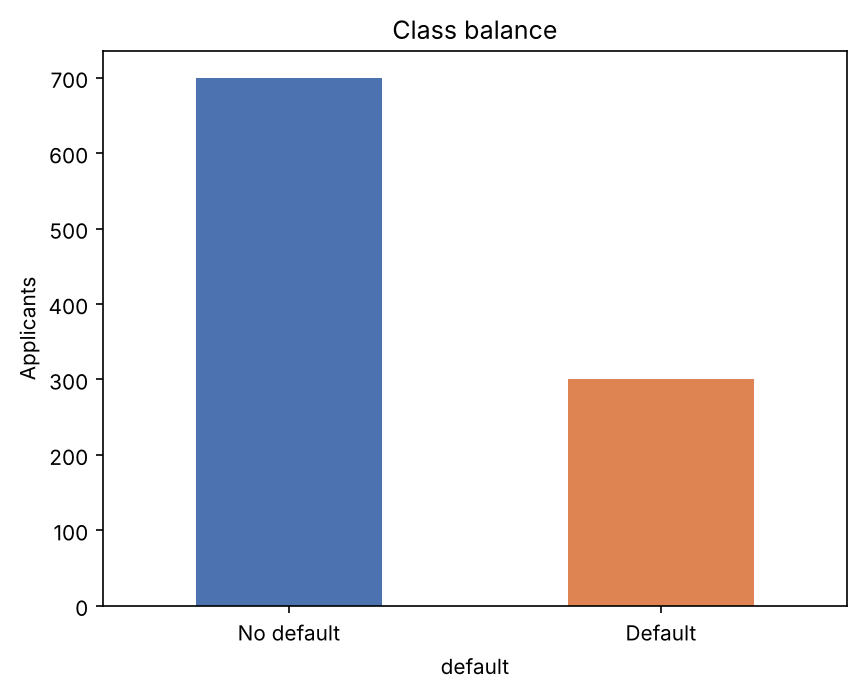
\includegraphics[width=0.42\textwidth]{class_balance.png}
\caption{Class balance: 700 applicants repaid and 300 defaulted.}
\label{fig:balance}
\end{figure}

% ---------- 4 ----------
\section{Data Preprocessing}

\subsection{Cleaning}

We checked four things.
\begin{enumerate}
  \item \textbf{Blank cells.} None.
  \item \textbf{Duplicate rows.} None.
  \item \textbf{Hidden missing values.} Some categories really mean ``the bank did not know''. Table~\ref{tab:hidden} shows that these rows behave differently from the rest. Unknown savings default much less than average, and unknown property defaults much more. So ``unknown'' carries signal. Filling it with the most common value would erase that signal, so we kept it as its own category.
  \item \textbf{Outliers.} We used the IQR rule: a value is an outlier if it lies below $Q_1 - 1.5\,\mathrm{IQR}$ or above $Q_3 + 1.5\,\mathrm{IQR}$, where $\mathrm{IQR} = Q_3 - Q_1$. Table~\ref{tab:outliers} shows that long and large loans are outliers, but they are real loans and they default at almost twice the normal rate of 30\%. Removing them would remove the riskiest applicants, so we kept them. For \texttt{num\_dependents}, $Q_1 = Q_3 = 1$, so every value of 2 is flagged. This shows that the IQR rule must not be applied blindly.
\end{enumerate}

\begin{table}[H]
\centering
\caption{Hidden missing values.}
\label{tab:hidden}
\begin{tabular}{lccc}
\toprule
Group & Rows & Default rate & Default rate (others) \\
\midrule
savings = unknown / none & 183 & 0.175 & 0.328 \\
property = unknown / none & 154 & 0.435 & 0.275 \\
\bottomrule
\end{tabular}
\end{table}

\begin{table}[H]
\centering
\caption{Outliers by the IQR rule (overall default rate is 0.30).}
\label{tab:outliers}
\begin{tabular}{lccc}
\toprule
Feature & Unique values & Outliers & Default rate of outliers \\
\midrule
duration\_months & 33 & 70 & 0.571 \\
credit\_amount & 921 & 72 & 0.542 \\
age & 53 & 23 & 0.261 \\
existing\_credits & 4 & 6 & 0.333 \\
num\_dependents & 2 & 155 & 0.297 \\
installment\_rate, residence\_since & 4 & 0 & -- \\
\bottomrule
\end{tabular}
\end{table}

\begin{figure}[H]
\centering
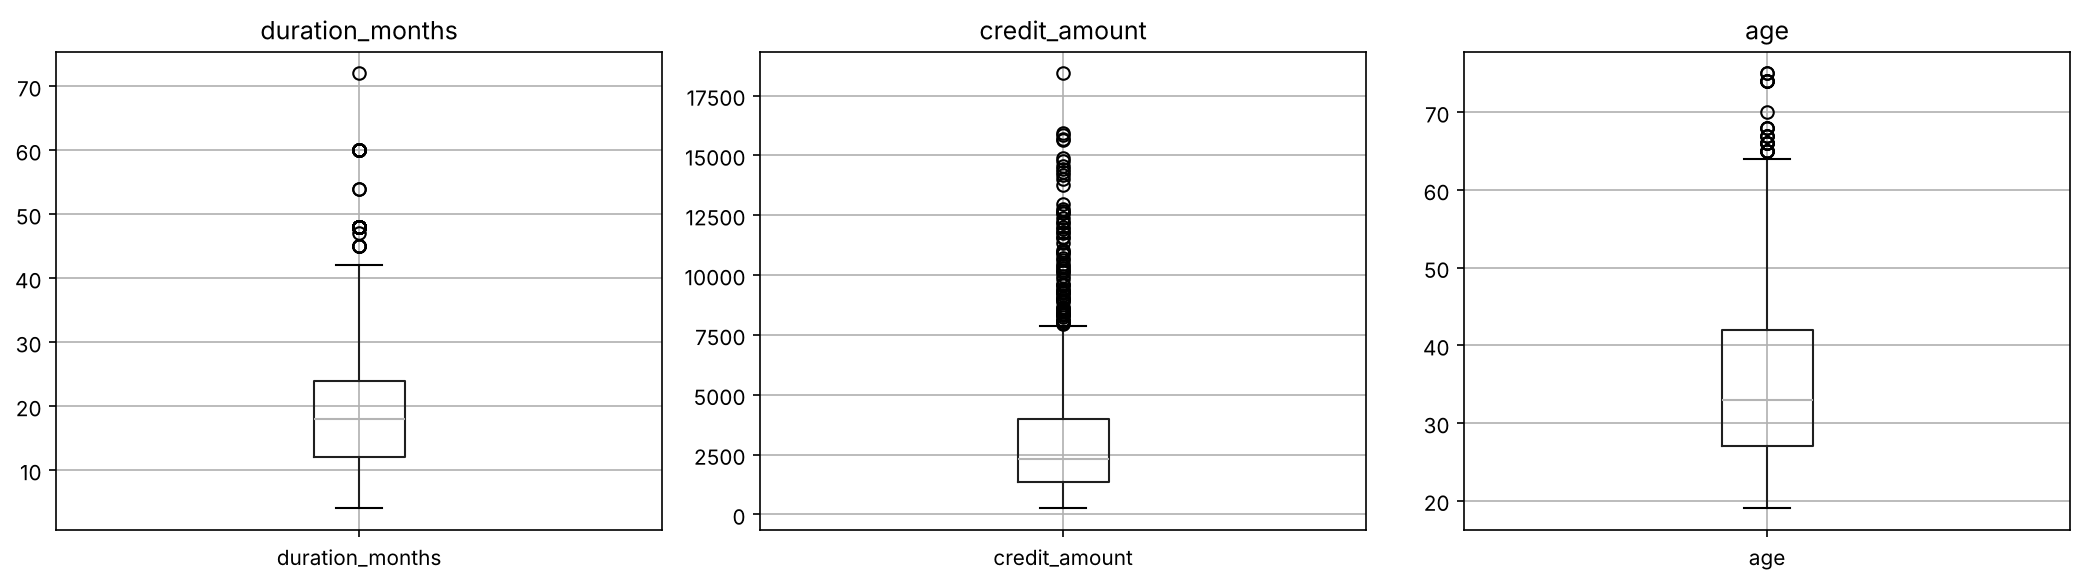
\includegraphics[width=0.95\textwidth]{outliers.png}
\caption{Boxplots of loan duration, credit amount and age. The points beyond the whiskers are the IQR outliers.}
\end{figure}

\subsection{Exploratory analysis}

Figure~\ref{fig:eda} shows that the features carry real signal. Applicants with a negative checking balance default far more often than applicants with no checking account, and defaulters take longer loans on average.

\begin{figure}[H]
\centering
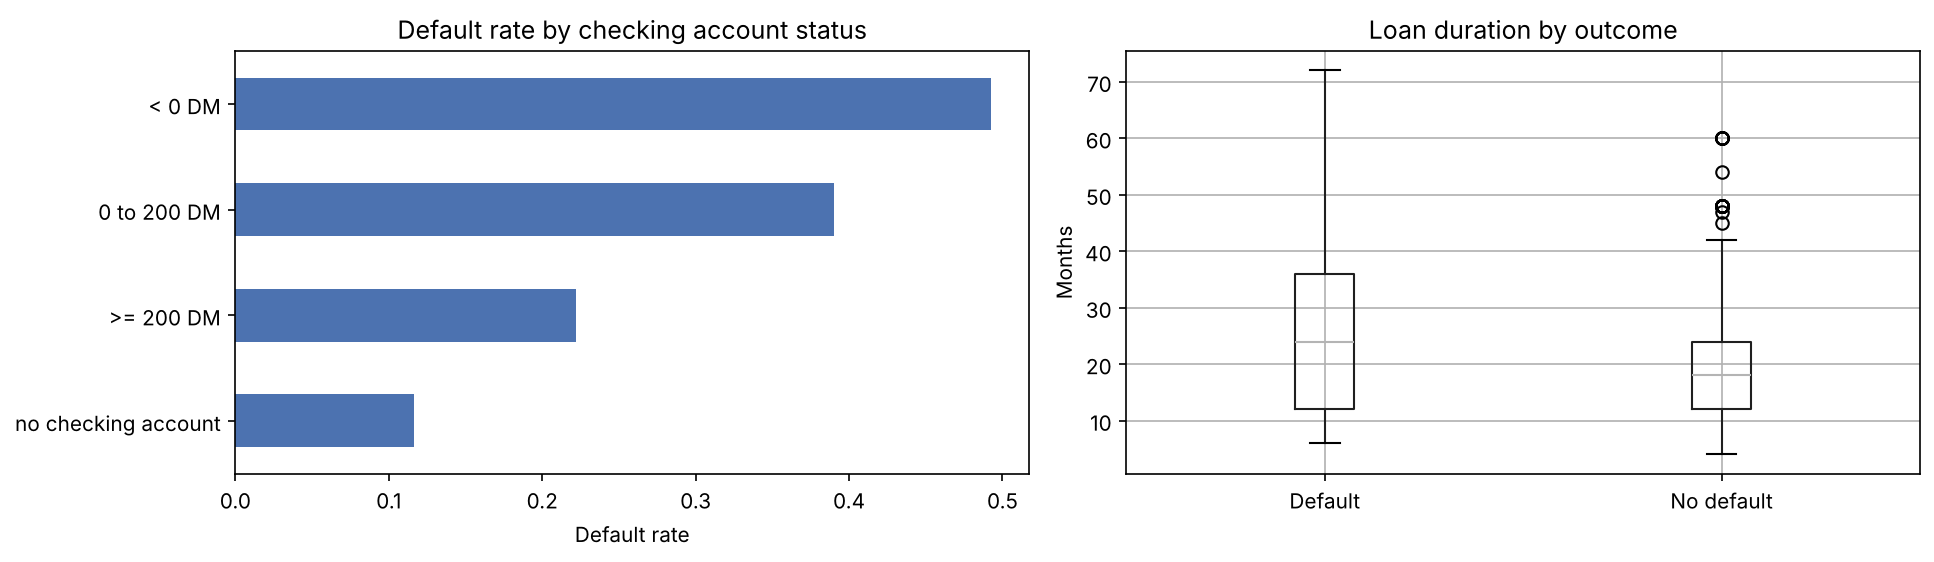
\includegraphics[width=0.98\textwidth]{eda.png}
\caption{Left: default rate by checking account status. Right: loan duration by outcome.}
\label{fig:eda}
\end{figure}

\subsection{Train/test split, scaling and encoding}

\begin{itemize}
  \item \textbf{Split.} 80/20 stratified split with a fixed random seed: 800 training rows and 200 test rows. Stratification keeps the 70/30 ratio in both sets, so the test set has exactly 60 defaulters.
  \item \textbf{Numeric features.} Median imputation, then standardisation $z = (x - \mu)/\sigma$, where $\mu$ and $\sigma$ are the mean and standard deviation of the training data.
  \item \textbf{Categorical features.} Most-frequent imputation, then one-hot encoding. Unknown categories at prediction time become an all-zero row instead of an error. After encoding there are 61 input columns.
  \item \textbf{No data leakage.} All steps sit inside a scikit-learn~\cite{sklearn} \texttt{Pipeline}. The imputers, scaler and encoder are fitted on the training data only. The data has no blanks, so the imputers change nothing here, but a new applicant with a missing field still gets a prediction.
\end{itemize}

% ---------- 5 ----------
\section{Machine Learning Algorithms}

We compare three classifiers of increasing flexibility~\cite{mitchell,alpaydin}.

\textbf{Logistic Regression.} A linear model that predicts the probability of default:
\begin{equation}
  P(y=1 \mid \mathbf{x}) = \sigma(\mathbf{w}^\top\mathbf{x} + b) = \frac{1}{1 + e^{-(\mathbf{w}^\top\mathbf{x} + b)}}
\end{equation}
where $\mathbf{x}$ is the applicant's feature vector, $\mathbf{w}$ the learned weights and $b$ the bias. An applicant is flagged as a defaulter when this probability is at least 0.5. Each feature has one weight, and a positive weight pushes towards default, so the model is easy to explain. We use \texttt{max\_iter=1000} so that the solver converges.

\textbf{Decision Tree.} The tree splits the data on one feature at a time and chooses the split that most reduces the Gini impurity $G = 1 - \sum_c p_c^2$, where $p_c$ is the share of class $c$ in a node. We cap the depth at 5 to limit overfitting.

\textbf{Random Forest.} An ensemble of 100 decision trees. Each tree is trained on a bootstrap sample of the rows and considers a random subset of features at each split. The forest averages the trees' votes, which reduces the variance of a single tree.

\textbf{Handling class imbalance.} By default, every training mistake counts the same, so the model learns mostly from the 70\% majority. We retrain every model with balanced class weights:
\begin{equation}
  w_c = \frac{n}{k\,n_c}
\end{equation}
where $n$ is the number of training rows, $k = 2$ is the number of classes and $n_c$ is the number of rows in class $c$. On the 800 training rows this gives $w_1 \approx 1.67$ for defaulters and $w_0 \approx 0.71$ for good applicants, so a mistake on a defaulter costs about 2.3 times more during training.

\textbf{Metrics.} Default is the positive class. TP, FP, TN and FN are the true positives, false positives, true negatives and false negatives.
\begin{gather}
  \text{Recall} = \frac{TP}{TP+FN}, \qquad
  \text{Specificity} = \frac{TN}{TN+FP}, \qquad
  \text{Precision} = \frac{TP}{TP+FP}, \\
  F_1 = \frac{2 \cdot \text{Precision} \cdot \text{Recall}}{\text{Precision} + \text{Recall}}
\end{gather}
Recall is the share of real defaulters that the model catches. Specificity is the share of good applicants that the model correctly approves.

% ---------- 6 ----------
\section{Workflow}

Figure~\ref{fig:workflow} shows the stages of the project from raw data to a prediction for a new applicant. The blue stages form the model pipeline. The orange stages are the two key decisions: balancing the class weights, and choosing the final model.

\begin{figure}[H]
\centering
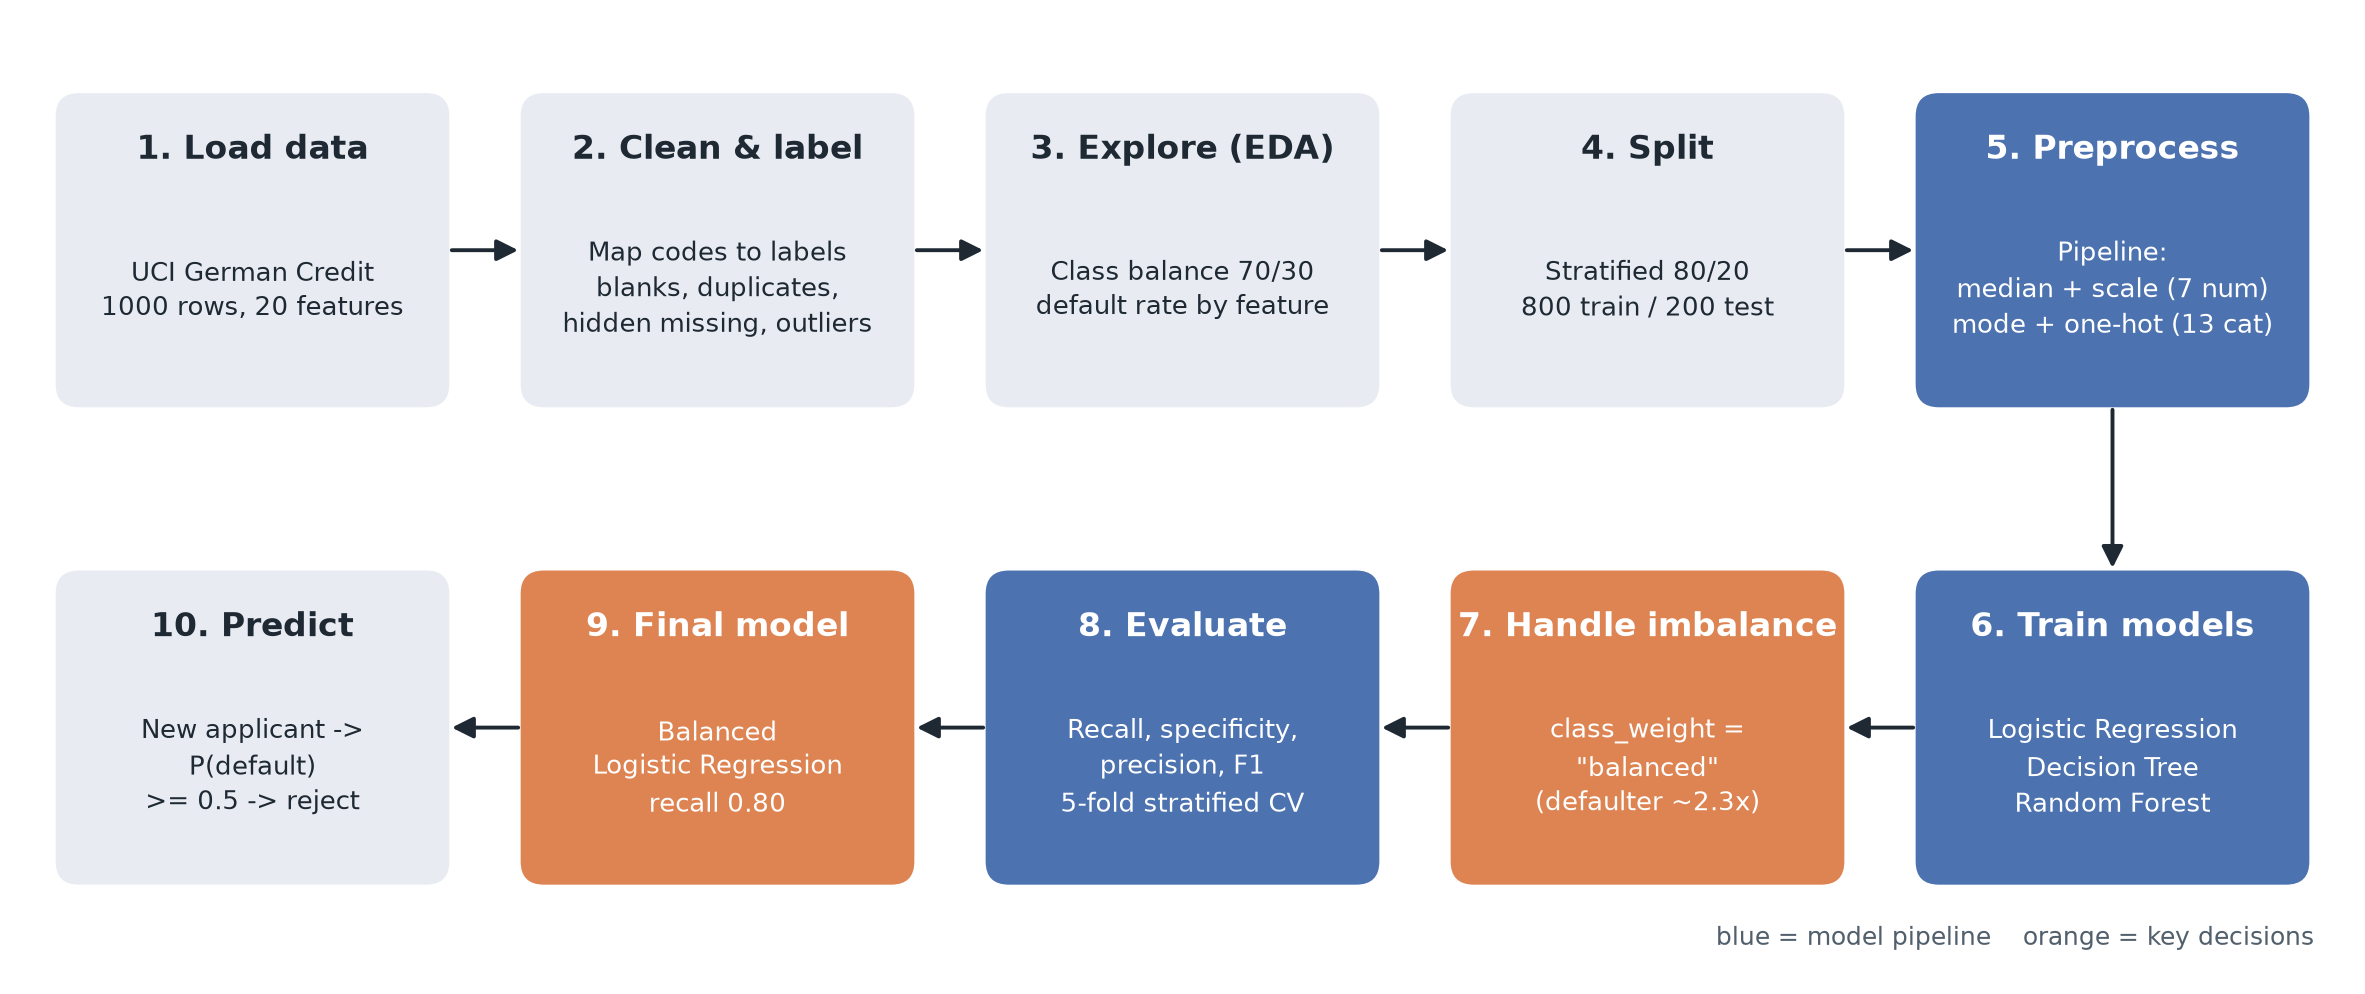
\includegraphics[width=\textwidth]{workflow.png}
\caption{Project workflow.}
\label{fig:workflow}
\end{figure}

% ---------- 7 ----------
\section{Experimental Results}

\subsection{Baseline and balanced models}

Table~\ref{tab:results} shows the test set results. The baseline models reach up to 78\% accuracy, but they catch at most about half of the defaulters. This is the accuracy trap: a model that always says ``no default'' would already score 70\%.

\begin{table}[H]
\centering
\caption{Test set results (200 rows, 60 defaulters) before and after balancing.}
\label{tab:results}
\begin{tabular}{llccccc}
\toprule
Setting & Model & Accuracy & Precision & Recall & Specificity & F1 \\
\midrule
\multirow{3}{*}{Baseline} & Logistic Regression & 0.780 & 0.667 & 0.533 & 0.886 & 0.593 \\
 & Decision Tree & 0.645 & 0.420 & 0.483 & 0.714 & 0.450 \\
 & Random Forest & 0.780 & 0.735 & 0.417 & 0.936 & 0.532 \\
\midrule
\multirow{3}{*}{Balanced} & Logistic Regression & 0.750 & 0.558 & \textbf{0.800} & 0.729 & \textbf{0.658} \\
 & Decision Tree & 0.570 & 0.377 & 0.667 & 0.529 & 0.482 \\
 & Random Forest & 0.770 & 0.617 & 0.617 & 0.836 & 0.617 \\
\bottomrule
\end{tabular}
\end{table}

\begin{table}[H]
\centering
\caption{Defaulters caught out of 60 on the test set.}
\begin{tabular}{lcc}
\toprule
Model & Baseline & Balanced \\
\midrule
Logistic Regression & 32 & \textbf{48} \\
Decision Tree & 29 & 40 \\
Random Forest & 25 & 37 \\
\bottomrule
\end{tabular}
\end{table}

Balancing raises recall for all three models. Logistic Regression goes from 0.53 to 0.80, so it catches 48 of the 60 defaulters instead of 32. The price is specificity, which falls from 0.89 to 0.73: the model now rejects 38 good applicants instead of 16. In lending this is the right trade. The Decision Tree gains recall but loses a lot of accuracy, so it is the weakest model. Random Forest gains the least.

\begin{figure}[H]
\centering
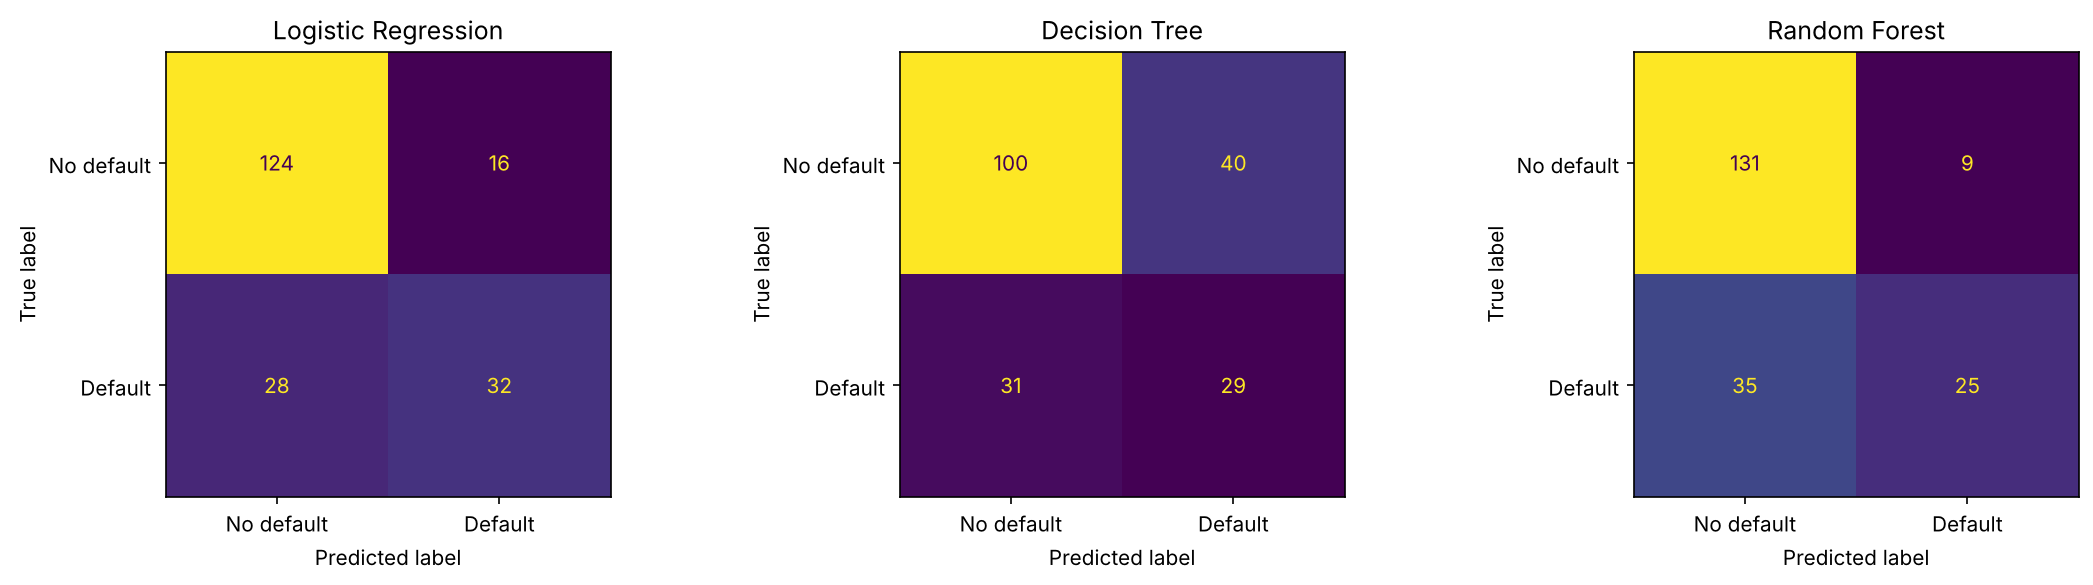
\includegraphics[width=0.98\textwidth]{cm_baseline.png}
\caption{Confusion matrices of the baseline models. The bottom-left cell is the number of missed defaulters.}
\end{figure}

\begin{figure}[H]
\centering
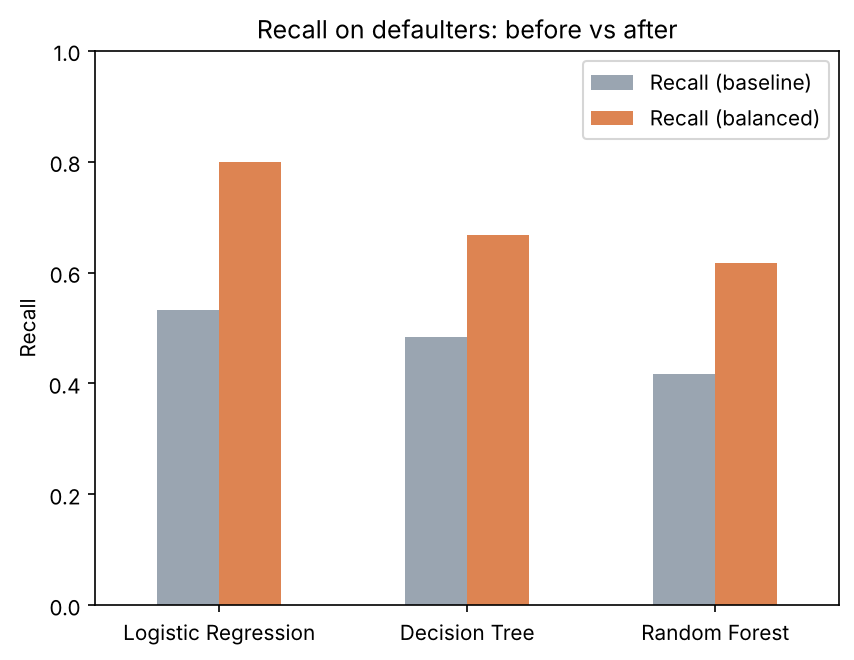
\includegraphics[width=0.46\textwidth]{recall_compare.png}\hfill
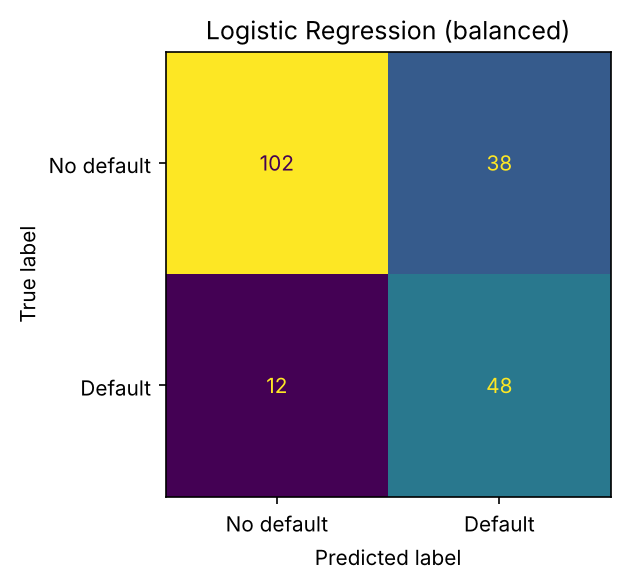
\includegraphics[width=0.40\textwidth]{cm_final.png}
\caption{Left: recall before and after balancing. Right: confusion matrix of the final model (balanced Logistic Regression): 48 of 60 defaulters caught, 12 missed.}
\label{fig:cm}
\end{figure}

\subsection{Cross-validation}

One 80/20 split has only 60 defaulters in the test set, so one lucky split could change the numbers a lot. We repeated the balanced training with 5-fold stratified cross-validation on all 1000 rows. The pipeline is refitted inside every fold, so there is no leakage.

\begin{table}[H]
\centering
\caption{5-fold stratified cross-validation with balanced weights (mean $\pm$ standard deviation).}
\label{tab:cv}
\small
\setlength{\tabcolsep}{4pt}
\begin{tabular}{lccccc}
\toprule
Model & Accuracy & Precision & Recall & Specificity & F1 \\
\midrule
Logistic Regression & 0.719 $\pm$ 0.027 & 0.524 $\pm$ 0.034 & \textbf{0.720} $\pm$ 0.041 & 0.719 $\pm$ 0.029 & \textbf{0.606} $\pm$ 0.034 \\
Decision Tree & 0.636 $\pm$ 0.037 & 0.435 $\pm$ 0.029 & 0.660 $\pm$ 0.077 & 0.626 $\pm$ 0.080 & 0.520 $\pm$ 0.021 \\
Random Forest & 0.735 $\pm$ 0.012 & 0.561 $\pm$ 0.022 & 0.547 $\pm$ 0.016 & 0.816 $\pm$ 0.018 & 0.553 $\pm$ 0.014 \\
\bottomrule
\end{tabular}
\end{table}

Cross-validated recall for Logistic Regression is 0.72, lower than the 0.80 on the single test split, but it is still clearly the best of the three models. The ranking does not change, so the conclusion holds.

\subsection{Final model and feature importance}

We chose balanced Logistic Regression as the final model. It has the best recall and F1, both on the test set and in cross-validation, and it is the easiest model to explain. A bank must be able to say why it rejected an application, and with Logistic Regression each feature has one weight.

\begin{figure}[H]
\centering
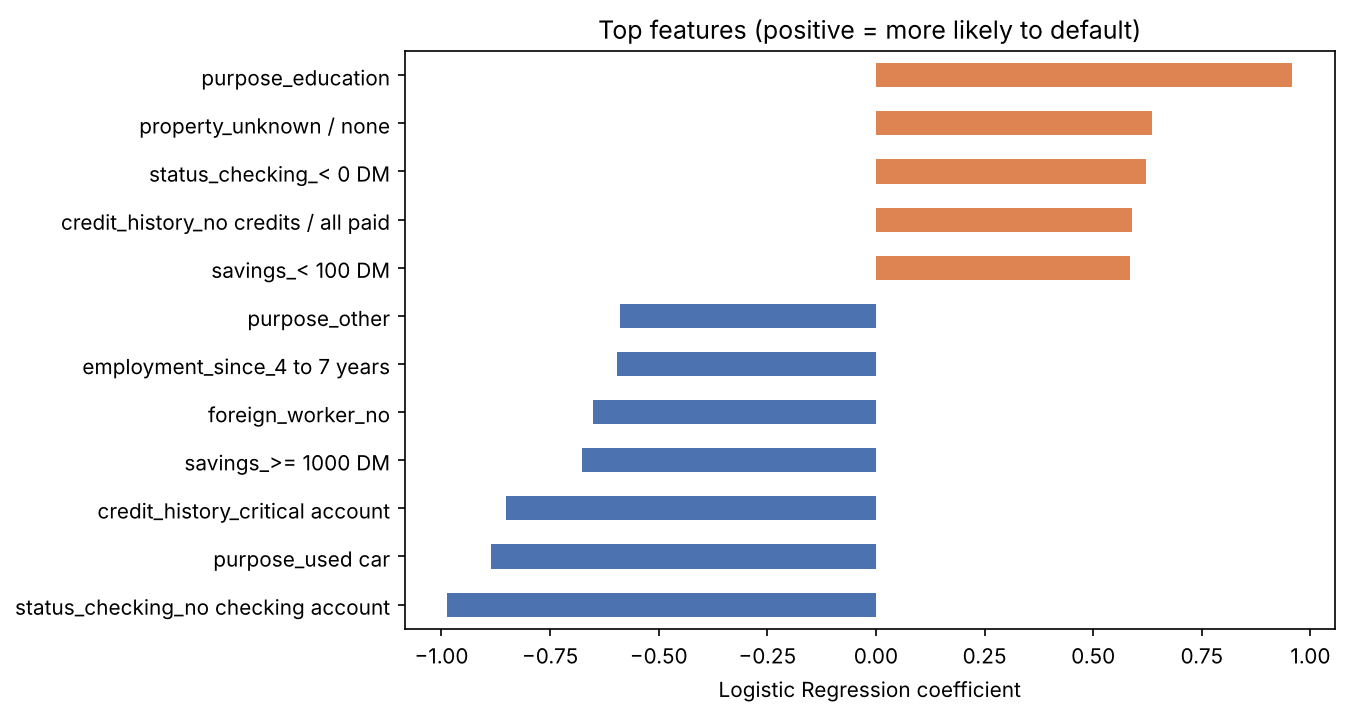
\includegraphics[width=0.7\textwidth]{top_features.png}
\caption{The 12 largest Logistic Regression coefficients. Positive values push towards default.}
\label{fig:features}
\end{figure}

A negative checking balance, savings under 100~DM, unknown property and loans for education raise the risk. Having no checking account at this bank, savings of 1000~DM or more, and a used-car loan lower it.

% ---------- 8 ----------
\section{Project Implementation / Screenshots}

The project is a single Jupyter notebook in Python, using pandas, matplotlib and scikit-learn. The code and data are on GitHub at \url{https://github.com/AabhasK/Credit-Risk-Predictor}.

\textbf{Loading the data.} The notebook reads the local file if it exists. Otherwise it downloads the dataset with \texttt{ucimlrepo}. The target is recoded so that 1 means default.

\begin{figure}[H]
\centering
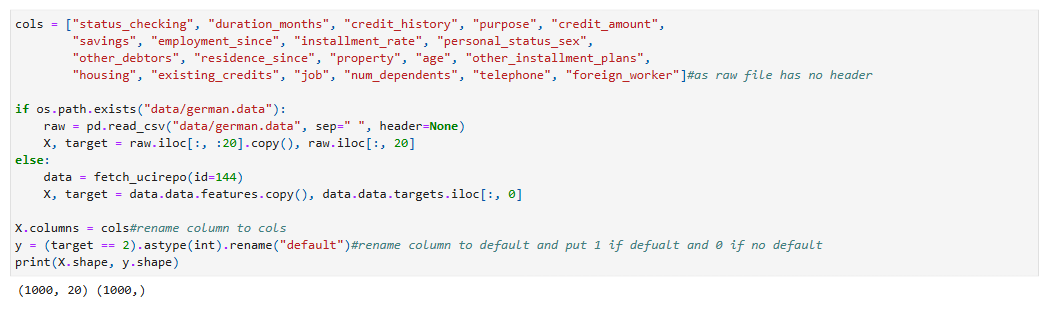
\includegraphics[width=\textwidth]{screens/ss_load.png}
\caption{Loading the data and recoding the target.}
\end{figure}

\begin{figure}[H]
\raggedright\textbf{Checking hidden missing values.}\par\smallskip
\centering
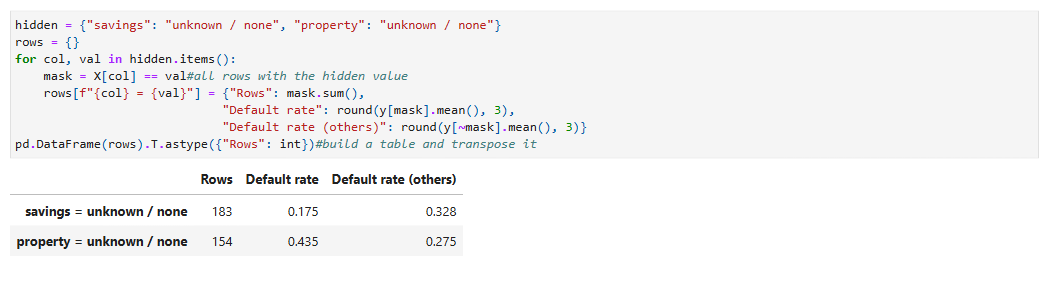
\includegraphics[width=\textwidth]{screens/ss_hidden.png}
\caption{Default rate of the ``unknown'' groups compared with all other rows.}
\end{figure}

\textbf{Preprocessing and models.} The preprocessing and the classifier are combined into one \texttt{Pipeline}, so that \texttt{fit} learns the scaler and encoder from the training data only.

\begin{lstlisting}
def make_prep():
    num = Pipeline([("impute", SimpleImputer(strategy="median")),
                    ("scale", StandardScaler())])
    cat = Pipeline([("impute", SimpleImputer(strategy="most_frequent")),
                    ("onehot", OneHotEncoder(handle_unknown="ignore"))])
    return ColumnTransformer([("num", num, num_cols), ("cat", cat, cat_cols)])

def make_models(class_weight=None):
    models = {
        "Logistic Regression": LogisticRegression(max_iter=1000, class_weight=class_weight),
        "Decision Tree": DecisionTreeClassifier(max_depth=5, class_weight=class_weight,
                                                random_state=42),
        "Random Forest": RandomForestClassifier(class_weight=class_weight, random_state=42),
    }
    return {name: Pipeline([("prep", make_prep()), ("clf", clf)])
            for name, clf in models.items()}
\end{lstlisting}

\begin{figure}[H]
\raggedright\textbf{Training with balanced weights.}\par\smallskip
\centering
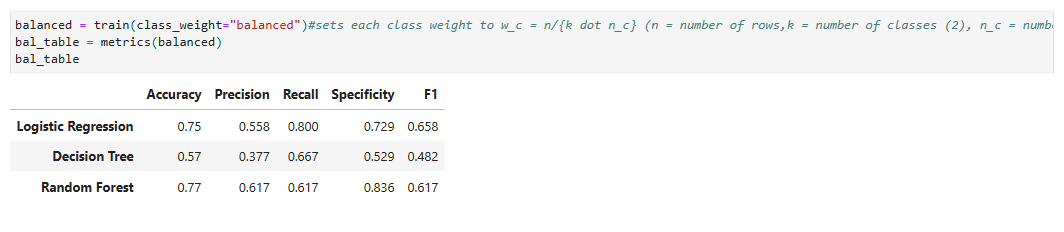
\includegraphics[width=\textwidth]{screens/ss_balanced.png}
\caption{Balanced models on the test set.}
\end{figure}

\begin{figure}[H]
\raggedright\textbf{Cross-validation.}\par\smallskip
\centering
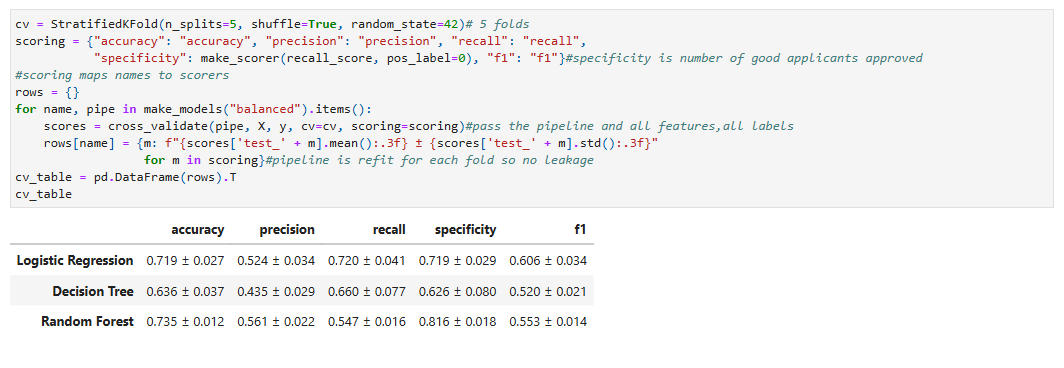
\includegraphics[width=\textwidth]{screens/ss_cv.png}
\caption{5-fold stratified cross-validation.}
\end{figure}

\textbf{Predicting a new applicant.} We start from a typical applicant (median of each numeric column, most common value of each categorical column) and make three risky changes: a 9000~DM loan, a 36-month term and a negative checking balance. All three balanced models score this applicant above 80\% default risk.

\begin{figure}[H]
\centering
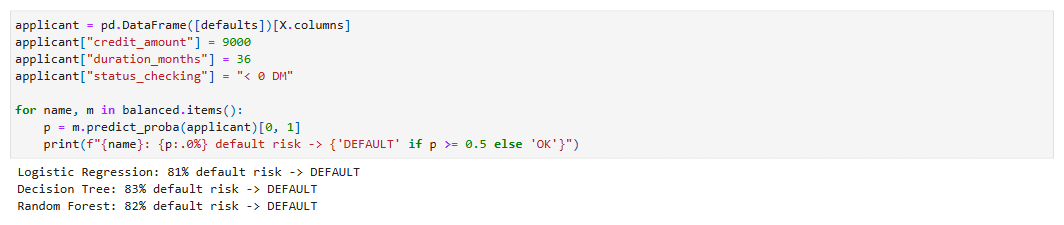
\includegraphics[width=\textwidth]{screens/ss_predict.png}
\caption{Default risk for a new applicant.}
\end{figure}

% ---------- 9 ----------
\section{Challenges and Limitations}

\textbf{Challenges.}
\begin{itemize}
  \item \textbf{Class imbalance.} With 70\% good applicants, the baseline models learned to favour ``no default'' and caught only about half of the defaulters. Balanced class weights fixed most of this.
  \item \textbf{Misleading accuracy.} Accuracy rewarded the wrong behaviour, so we had to choose recall and specificity as the main metrics.
  \item \textbf{Hidden missing values and outliers.} The usual fixes (fill with the mode, drop the outliers) would have removed useful signal. We checked the default rate of each group before deciding to keep them.
  \item \textbf{Small test set.} 60 defaulters in the test set make single-split results noisy. Cross-validation was needed to trust the ranking.
\end{itemize}

\textbf{Limitations.}
\begin{itemize}
  \item \textbf{Small, old dataset.} 1000 loans from one German bank in the 1990s may not represent today's borrowers.
  \item \textbf{Fixed threshold.} We used a 0.5 cut-off. The best threshold depends on the real cost of each error, which we do not know.
  \item \textbf{Sensitive attributes.} The data contains sex, marital status and foreign-worker status. A real credit model should not use these features, and should be audited for fairness.
  \item \textbf{Counter-intuitive weights.} Some coefficients are surprising. For example, a ``critical account'' credit history lowers the predicted risk. Logistic Regression shows correlation in this data, not cause.
  \item \textbf{Limited tuning.} We did not tune hyperparameters beyond the tree depth.
\end{itemize}

% ---------- 10 ----------
\section{Conclusion and Future Scope}

\textbf{Conclusion.} Accuracy hides the real problem in imbalanced credit data. By measuring recall on defaulters and training with balanced class weights, we raised the share of defaulters caught by Logistic Regression from 53\% to 80\% on the test set (72\% in cross-validation). Specificity fell from 0.89 to 0.73, which is an acceptable trade in lending. Balanced Logistic Regression is our final model: it has the best recall and F1 of the three models, and every decision can be explained through its weights.

\textbf{Future scope.}
\begin{itemize}
  \item Tune the decision threshold with a cost matrix (for example, a missed defaulter costs 5 times a rejected good applicant).
  \item Remove sensitive attributes and measure fairness across groups.
  \item Try gradient boosting (XGBoost, LightGBM) and tune hyperparameters with cross-validation.
  \item Use ROC-AUC and precision-recall curves for threshold-free comparison.
  \item Test on a larger and more recent credit dataset, and deploy the model as a simple web form for credit officers.
\end{itemize}

\begin{thebibliography}{9}
\bibitem{uci} H.~Hofmann, \emph{Statlog (German Credit Data)}, UCI Machine Learning Repository, 1994. \url{https://doi.org/10.24432/C5NC77}
\bibitem{sklearn} F.~Pedregosa et al., ``Scikit-learn: Machine Learning in Python,'' \emph{JMLR}, vol.~12, pp.~2825--2830, 2011.
\bibitem{mitchell} T.~Mitchell, \emph{Machine Learning}, McGraw Hill, 1997.
\bibitem{alpaydin} E.~Alpaydin, \emph{Introduction to Machine Learning}, 3rd ed., MIT Press, 2014.
\end{thebibliography}

\end{document}
